\documentclass[a4paper,12pt]{article}
 		
\usepackage{cmap}	

\usepackage[T2A]{fontenc}

\usepackage[utf8x]{inputenc}


\usepackage[english,russian]{babel}	

		


\usepackage[
bookmarks=true, colorlinks=true, unicode=true,
urlcolor=black,linkcolor=black, anchorcolor=black,
citecolor=black, menucolor=black, filecolor=black,
]{hyperref}

\usepackage{color}
\usepackage{caption}
\DeclareCaptionFont{white}{\color{black}}
\DeclareCaptionFormat{listing}{\colorbox{white}{\parbox{\textwidth}{#1#2#3}}}
\captionsetup[lstlisting]{format=listing,labelfont=white,textfont=white}

\usepackage{amsmath,amsfonts,amssymb,amsthm,mathtools} 
\usepackage{wasysym}

\usepackage{graphicx}
%\usepackage[cache=false]{minted}

\usepackage{indentfirst}

\usepackage{listings} 
\usepackage{fancyvrb}


\usepackage{geometry}
\geometry{left=2cm}
\geometry{right=1.5cm}
\geometry{top=1cm}
\geometry{bottom=2cm}

\setlength{\parindent}{5ex}
\setlength{\parskip}{0.5em}


\begin{document}
\lstset{ %
	language=Python,                 % выбор языка для подсветки (здесь это С)
	basicstyle=\small\sffamily, % размер и начертание шрифта для подсветки кода
	numbers=left,               % где поставить нумерацию строк (слева\справа)
	numberstyle=\tiny,           % размер шрифта для номеров строк
	stepnumber=1,                   % размер шага между двумя номерами строк
	numbersep=5pt,                % как далеко отстоят номера строк от подсвечиваемого кода
	backgroundcolor=\color{white}, % цвет фона подсветки - используем \usepackage{color}
	showspaces=false,            % показывать или нет пробелы специальными отступами
	showstringspaces=false,      % показывать или нет пробелы в строках
	showtabs=false,             % показывать или нет табуляцию в строках
	frame=single,              % рисовать рамку вокруг кода
	tabsize=2,                 % размер табуляции по умолчанию равен 2 пробелам
	captionpos=t,              % позиция заголовка вверху [t] или внизу [b] 
	breaklines=true,           % автоматически переносить строки (да\нет)
	breakatwhitespace=false, % переносить строки только если есть пробел
	escapeinside={\%*}{*)}   % если нужно добавить комментарии в коде
}

% Титульный лист
\large
\begin{center}
	Федеральное государственное бюджетное образовательное учреждение 
	высшего образования <<Московский государственный технический 
	университет имени Н. Э. Баумана>> 
	(национальный исследовательский университет)
\end{center}

\vspace*{30mm} 

\huge
\begin{center}
	Дисциплина: <<Анализ алгоритмов>>
	
	Отчет по лабораторной работе №6
\end{center}

\vspace*{30mm} 

\huge
\begin{center}
	Тема работы:\\
	<<Задача коммивояжера.\\ Муравьиный алгоритм>>
\end{center}
\vspace*{30mm} 

\large
\begin{flushright}
	Студент: Левушкин И. К. \\
	Группа: ИУ7-52Б \\
	Преподаватели: Волкова Л. Л., \\ Строганов Ю. В. \\
\end{flushright}

\vspace*{40mm}
\begin{center}
	Москва, 2019 г.  
\end{center}
\thispagestyle{empty}

\tableofcontents
% \setcounter{page}{1}

\section*{Введение}
\addcontentsline{toc}{section}{Введение}

Задача коммивояжера занимает особое место в комбинаторной оптимизации и 
исследовании операций. Она формулируется как задача поиска минимального по стоимости замкнутого 
маршрута по всем вершинам
без повторений на полном взвешенном графе. Содержательно вершины 
графа являются
городами, которые должен посетить коммивояжер, а веса ребер отражают расстояния 
(длины) или стоимости
проезда. Эта задача является NP-трудной, и точный переборный алгоритм её решения 
имеет факториальную
сложность. ~\cite{kom}

Решение данной задачи важно в первую очередь для крупных
транспортных компаний, которые стремятся оптимизировать перевозки
и минимизировать расходы. ~\cite{pract}

Особый интерес представляет муравьиный алгоритм,
способный эффективно находить приближенное решение задачи коммивояжера.

\textbf{Цель лабораторной работы:} изучение подходов к решению задачи коммивояжера
на материале алгоритма полного перебора и муравьиного алгоритма.

\textbf{Задачи работы:}

\begin{enumerate} 
	\item[1)] изучить муравьиный алгоритм;
	\item[2)] применить метод динамического программирования для  
	реализации муравьиного алгоритма и полного перебора;
	\item[3)] экспериментально подтвердить различия во временнóй эффективности алгоритмов 
	при помощи разработанного программного обеспечения на материале замеров процессорного 
	времени;
	\item[4)] провести параметризацию муравьиного алгоритма;
	\item[5)] описать и обосновать полученные результаты в отчете о лабораторной 
	работе, выполненного как расчётно-пояснительная записка. 
\end{enumerate} 
\pagebreak

\section{Аналитический раздел}

В данном разделе будет рассмотрен муравьиный алгоритм.

\subsection{Описание алгоритмов}

\subsubsection{Муравьиный алгоритм}

Идея муравьиного алгоритма – моделирование поведения муравьёв, связанного с их способностью быстро
находить кратчайший путь от муравейника к источнику пищи и адаптироваться к изменяющимся условиям,
находя новый кратчайший путь. При своём движении муравей метит путь феромоном, и эта информация
используется другими муравьями для выбора пути. Это элементарное правило поведения и определяет
способность муравьёв находить новый путь, если старый оказывается недоступным.
~\cite{stovba}

У муравья есть 3 чувства: 

\begin{enumerate}
	\item Обоняние --- муравей чует феромон и его концентрацию на ребре. 
	\item Зрение --- муравей оценивает длину ребра. 
	\item Память --- муравей запоминает посещенные города.  
\end{enumerate}

При старте матрица феромонов $\tau$ инициализируется равномерно некоторой константой. 

Если муравей \textit{k} находится в городе \textit{i} и выбирает куда пойти, то делает это по вероятностному правилу: 

\begin{equation}
P_{ij}(t) =  \left\{
\begin{aligned}
&\frac{{\tau_{ij}(t)}^{\alpha} \eta_{ij}^{\beta}}{\sum_{q=1}^m {\tau_{iq}(t)}^{\alpha} \eta_{iq}^{\beta}}, &если j не посещен,\\
&0, &иначе,
\end{aligned}
\right.
\label{p0}
\end{equation}

где\\

$\alpha, \beta$ -- весовые коэффициенты, которые задают важность феромона и привлекательность ребра, $\alpha + \beta = const$, \\
$\eta_{iq} = \frac{1}{d_{ij}}$ -- привлекательность ребра (города),\\
$d_{ij}$ -- длина ребра.

Кроме того, надо учитывать изменение феромона по формуле 2: 

\begin{equation} \tau (t+1)=\tau_{ij}(t)\cdot(1-\rho)+\sum_{k=1}^n\Delta \tau_{k,ij}(t), \end{equation}

\begin{equation}
\Delta \tau_{k,ij}(t) =  
\left\{
\begin{aligned}
&\frac{Q}{L_k}, & если ребро ij в маршруте,\\
&0, & иначе,
\end{aligned}
\right.
\end{equation}

где\\

$L_k$ -- длина маршрута \textit{k}-ого муравья,

$\rho$ -- коэффициент испарения феромона,

$Q$ -- нормировочная константа порядка длины наилучшего маршрута.



\subsection*{Выводы}
\addcontentsline{toc}{subsection}{Выводы}

Рассмотрен муравьиный алгоритм, выделены ключевые моменты его работы.


\section{Конструкторский раздел}

В разделе приводится псевдокод муравьиного алгоритма.

\subsection{Разработка алгоритмов}

Псевдокод муравьиного алгоритма для решения задачи коммивряжера:

\begin{flushleft}
	1. Ввод матрицы расстояний $D$\\
		2. Инициализация рёбер -- присвоение видимости $\eta_{ij}$ и начальной концентрации
		феромона\\
		3. Размещение муравьёв в случайно выбранные города без совпадений\\
		4. Выбор начального кратчайшего маршрута и определение $L^{*}$\\
		5. Цикл по времени жизни колонии t=1,tmax\\
		6. \hspace{1.5cm} Цикл по всем муравьям k=1,m\\
		7. \hspace{3cm}Построить маршрут $T_{k}(t)$ по правилу (1)\\
		8. \hspace{3cm}Рассчитать длину $L_{k}(t)$\\
		9. \hspace{1.5cm}Конец цикла по муравьям\\
		10. \hspace{1.5cm}Проверка всех $L_{k}(t)$ на лучшее решение по сравнению с $L*$\\
		11. \hspace{3cm}В случае если решение $L_{k}(t)$ лучше, обновить $L*$ и $T*$\\
		12. \hspace{1.5cm}Цикл по всем рёбрам графа\\
		13. \hspace{3cm}Обновить следы феромона на ребре согласно (2), (3)\\
		14. \hspace{1.5cm}Конец цикла по рёбрам\\
		15. Конец цикла по времени\\
		16. Вывести кратчайший маршрут $T*$ и его длину $L*$\\
\end{flushleft}

%На рис. \ref{fig:n1}-\ref{fig:n2} приведена 
%функциональная схема 
%муравьиного алгоритма.

\pagebreak

%\begin{figure}[h!]
%	\begin{center}
%		{\includegraphics[width = \textwidth]{img/n1.png}}
%		\caption{Муравьиный алгоритм для решения задачи коммивояжера}
%		\label{fig:n1}
%	\end{center}
%\end{figure}

%\begin{figure}[h!]
%	\begin{center}
%		{\includegraphics[width = \textwidth]{img/n2.png}}
%		\caption{Главный цикл муравьиного алгоритма}
%		\label{fig:n2}
%	\end{center}
%\end{figure}

\subsection*{Выводы}
\addcontentsline{toc}{subsection}{Выводы}

В разделе представлен пошаговый разбор
муравьиного алгоритма для решения задачи коммивояжера.


\section{Технологический раздел}

Здесь описываются требования к программному 
обеспечению и средства реализации, приводятся листинги 
программы и тестовые данные.

\subsection{Требования к программному обеспечению}

\begin{flushleft}
	\textbf{Входные данные:} 
	\begin{itemize}
		\item количество городов (целое число, большее 2).
	\end{itemize}
	
	\textbf{Выходные данные:} длины кратчайшего пути, маршруты,
	найденные полным перебором
	или муравьиным алгоритмом.
\end{flushleft}

\subsection{Средства реализации}

Программа написана на языке Python ~\cite{python}, который 
предоставляет программисту мощные инструменты для реализации различных алгоритмов и является достаточно 
надежным, эффективным и удобным для реализации сложных алгоритмов. Для написания использовался 
редактор исходного кода \textit{PyCharm} ~\cite{pycharm}.

Замер времени выполнения программы 
производится с помощью функции \textit{process\_time()} из библиотеки \textit{time},
функционал которой позволяет подсчитывать процессорное время в тиках,
а затем конвертировать полученный результат в секунды.

\subsection{Листинг программы}

Реализованная программа представлена
в листингах \ref{lst1}-\ref{lst2}.

\begin{lstlisting}[label=lst1,caption=Реализация полного перебора для решения задачи коммивояжера]
def calc_min_way(min_way, d_matrix, city_visit, i, j, way):
	if (i != -1):
		way += d_matrix[i][j]
		city_visit[j] = True
	
	count = 0
	for k in range(len(d_matrix)):
		if (not city_visit[k]):
			min_way = min(min_way, calc_min_way(min_way, d_matrix, city_visit[:], j, k, way))
		else:
			count += 1
	
	if (count == len(d_matrix)):
		return way
	
	return min_way

def get_min_way(min_way, d_matrix, city_visit):
	for i in range(len(d_matrix)):
		visit = city_visit[:]
		visit[i] = True
		min_way = min(min_way, calc_min_way(min_way, d_matrix, visit, -1, i, 0))
	return min_way


def full_search(d_matrix):
	min_way = 1000000
	min_way = get_min_way(min_way, d_matrix, [False for i in range(len(d_matrix))])
	return min_way
\end{lstlisting}

\begin{lstlisting}[label=lst2,caption=Реализация муравьиного алгоритма для решения задачи коммивояжера]
from random import *

class Ant(object):
	def __init__(self, i, towns_count):
		self.city_visit = [False for i in range(towns_count)]
		self.city_visit[i] = True
		self.edge_visit = []
		self.hole_way = 0
		self.position = i
	
	def get_edge_length(self, d_matrix, j):
		return d_matrix[self.position][j]
	
	def was(self, i):
		return self.city_visit[i]
	
	def move_ant(self, i, d_matrix):
		self.hole_way += d_matrix[self.position][i]
		self.edge_visit.append([self.position, i])
		self.position = i
		self.city_visit[i] = True



def calc_q(d_matrix):
	sum = 0
	count = 0
	for i in d_matrix:
		for j in i:
			sum += j
			count += 1
	
	return sum / count * len(d_matrix)

def create_pheromon_matrix(d_matrix, q):
	L = []
	for i in range(len(d_matrix)):
		L1 = []
		for j in range(len(d_matrix[i])):
			if (i == j):
				L1.append(0)
			else:
				L1.append(q / d_matrix[i][j])
		L.append(L1)
	return L


def random_way_choice(cities_probability):
	seed()
	rand_number = random()
	k = -1
	current_prob = 0
	for i in range(len(cities_probability)):
		current_prob += cities_probability[i]
		if (rand_number < current_prob):
			k = i
			break
	if (k == -1):
	for i in range(len(cities_probability)):
		if (cities_probability[i] > 0.000001):
			k = i
	return k

def move_ant(town, ant, d_matrix):
	ant.move_ant(town, d_matrix)


def calc_etta(d_matrix, i, j, ant):
	if (ant.was(j)):
		return 0
	return 1 / d_matrix[i][j]
	
def calc_town_probability(ant, pheromon_matrix, d_matrix, alpha, j):
	if (ant.was(j)):
		return 0
	
	betta = 1 - alpha
	
	znam = 0
	for i in range(len(d_matrix)):
		znam += (pheromon_matrix[ant.position][i] ** alpha) * (calc_etta(d_matrix, ant.position, i, ant) ** betta)
	
	p = ((pheromon_matrix[ant.position][j] ** alpha) * (calc_etta(d_matrix, ant.position, j, ant) ** betta) /
	znam)
	
	return p



def create_hole_way(ant, pheromon_matrix, d_matrix, alpha):
for i in range(len(d_matrix) - 1):
	cities_probability = []
	for j in range(len(d_matrix)):
		cities_probability.append(calc_town_probability(ant, pheromon_matrix, d_matrix, alpha, j))
	town = random_way_choice(cities_probability)
	move_ant(town, ant, d_matrix)



def edge_belong_to_ant_way(i, j, ant):
	for k in range(len(ant.edge_visit)):
		if (ant.edge_visit[k][0] == i and ant.edge_visit[k][1] == j):
			return True
	return False

def refresh_pheromon_matrix(pheromon_matrix, p, q, ants, d_matrix):
	one_minus_p = 1 - p
	for i in range(len(pheromon_matrix)):
		for j in range(len(pheromon_matrix)):
			sum_pheromons = 0
			for k in range(len(ants)):
				if (edge_belong_to_ant_way(i, j, ants[k])):
					sum_pheromons += q / ants[k].hole_way
			pher = pheromon_matrix[i][j] * one_minus_p + sum_pheromons
			if (i == j):
				pher = 0
			elif (pher < q / d_matrix[i][j]):
				pher = q / d_matrix[i][j]
			pheromon_matrix[i][j] = pher


def ants_algorythm(d_matrix):

	alpha = float(input("alpha: "))
	p = float(input("p: "))
	t_max = int(input("t_max: "))
	
	q = calc_q(d_matrix)
	best_hole_way = 1000000
	best_way = []
	
	pheromon_matrix = create_pheromon_matrix(d_matrix, q)
	
	for t in range(t_max):
		ants = []
		for i in range(len(d_matrix)):
			ant = Ant(i, len(d_matrix))
			ants.append(ant)
	
		for i in range(len(ants)):
			create_hole_way(ants[i], pheromon_matrix, d_matrix, alpha)
			if (ants[i].hole_way < best_hole_way):
				best_hole_way = ants[i].hole_way
				best_way = ants[i].edge_visit
	
		refresh_pheromon_matrix(pheromon_matrix, p, q, ants, d_matrix)
	print(best_way)
	return best_hole_way
\end{lstlisting}


\subsection{Тестовые данные}
\label{fig:test_data}

Тестирование полного перебора производится на следующей матрице
размерностью 10 (\textit{i} -- номер строки,
\textit{j} -- номер столбца):

\begin{table} [h!]
	\begin{center}
		\caption{Матрица}
		\begin{tabular}{|r|r|r|r|r|r|r|r|r|r|r|}
			\hline
			{\bf ij} &    {\bf 1} &    {\bf 2} &    {\bf 3} &    {\bf 4} &    {\bf 5} &    {\bf 6} &    {\bf 7} &    {\bf 8} &    {\bf 9} &   {\bf 10} \\
			\hline
			{\bf 1}& 0 & 3 & 10 & 2 & 5 & 2 & 8 & 8 & 8 & 7\\
			\hline
			{\bf 2}& 3 & 0 & 4 & 2 & 8 & 1 & 7 & 7 & 10 & 1\\
			\hline
			{\bf 3}& 10 & 4 & 0 & 8 & 5 & 4 & 10 & 2 & 6 & 1\\
			\hline
			{\bf 4}& 2 & 2 & 8 & 0 & 1 & 1 & 9 & 1 & 7 & 4\\
			\hline
			{\bf 5}& 5 & 8 & 5 & 1 & 0 & 7 & 1 & 9 & 4 & 8\\
			\hline
			{\bf 6}& 2 & 1 & 4 & 1 & 7 & 0 & 8 & 9 & 4 & 6\\
			\hline
			{\bf 7}& 8 & 7 & 10 & 9 & 1 & 8 & 0 & 4 & 4 & 8\\
			\hline
			{\bf 8}& 8 & 7 & 2 & 1 & 9 & 9 & 4 & 0 & 5 & 1\\
			\hline
			{\bf 9}& 8 & 10 & 6 & 7 & 4 & 4 & 4 & 5 & 0 & 7\\
			\hline
			{\bf 10}& 7 & 1 & 1 & 4 & 8 & 6 & 8 & 1 & 7 & 0\\
			\hline
		\end{tabular}  
		\label{m1}
	\end{center}
\end{table}

Полный перебор:
\begin{enumerate}
	\item Путь: $( 0 \rightarrow 5 \rightarrow 1 \rightarrow 9 \rightarrow 2 \rightarrow 7 \rightarrow 3 \rightarrow 4 \rightarrow 6 \rightarrow 8 )$
	\item Минимальный путь: 14
\end{enumerate}


Муравьиный алгоритм:

\begin{enumerate}
	\item $\alpha$ = 0.3; $\rho$ = 0.3; t\_max = 100
	\begin{enumerate}
		\item Путь: $( 7 \rightarrow 2 \rightarrow 9 \rightarrow 1 \rightarrow 5 \rightarrow 0 \rightarrow 3 \rightarrow 4 \rightarrow 6 \rightarrow 8 )$
		\item Минимальный путь: 15
	\end{enumerate}
	\item $\alpha$ = 0.4; $\rho$ = 0.5; t\_max = 100
	\begin{enumerate}
		\item Путь: $( 0 \rightarrow 3 \rightarrow 5 \rightarrow 1 \rightarrow 9 \rightarrow 2 \rightarrow 7 \rightarrow 6 \rightarrow 4 \rightarrow 8 )$
		\item Минимальный путь: 17
	\end{enumerate}
	\item $\alpha$ = 0.2; $\rho$ = 0.6; t\_max = 90
	\begin{enumerate}
		\item Путь: $( 8 \rightarrow 5 \rightarrow 0 \rightarrow 1 \rightarrow 9 \rightarrow 2 \rightarrow 7 \rightarrow 3 \rightarrow 4 \rightarrow 6 )$
		\item Минимальный путь: 16
	\end{enumerate}
	\item $\alpha$ = 0.6; $\rho$ = 0.45; t\_max = 120
	\begin{enumerate}
		\item Путь: $( 0 \rightarrow 5 \rightarrow 1 \rightarrow 2 \rightarrow 9 \rightarrow 7 \rightarrow 3 \rightarrow 4 \rightarrow 6 \rightarrow 8 )$
		\item Минимальный путь: 16
	\end{enumerate}
	\item $\alpha$ = 0.4; $\rho$ = 0.4; t\_max = 200
	\begin{enumerate}
		\item Путь: $( 8 \rightarrow 6 \rightarrow 4 \rightarrow 3 \rightarrow 7 \rightarrow 9 \rightarrow 2 \rightarrow 1 \rightarrow 5 \rightarrow 0 )$
		\item Минимальный путь: 16
	\end{enumerate}
\end{enumerate}



\subsection*{Выводы}
\addcontentsline{toc}{subsection}{Выводы}

В данном разделе были рассмотрены требования к 
программному обеспечению, обоснован выбор средств 
реализации, приведены листинги программы и тестовые 
данные. Все заявленные тесты успешно пройдены муравьиным алгоритмом и полным перебором.

\section{Исследовательский раздел}

В разделе представлены примеры выполнения программы,
результаты сравнения
алгоритмов решения задачи коммивояжера,
а также исследование \\ эффективности
поиска муравьиным алгоритмом при различных параметрах.

\subsection{Примеры работы}

%На рис. \ref{fig:t0}-\ref{fig:t1} приведены примеры работы программы. 

%\begin{figure}[h!]
%	\center{\includegraphics[scale = 0.7]{img/0.png}}
%	\caption{
%		Обработка некорректного ввода}
%	\label{fig:t0}
%\end{figure}

%\begin{figure}[h!]
%	\center{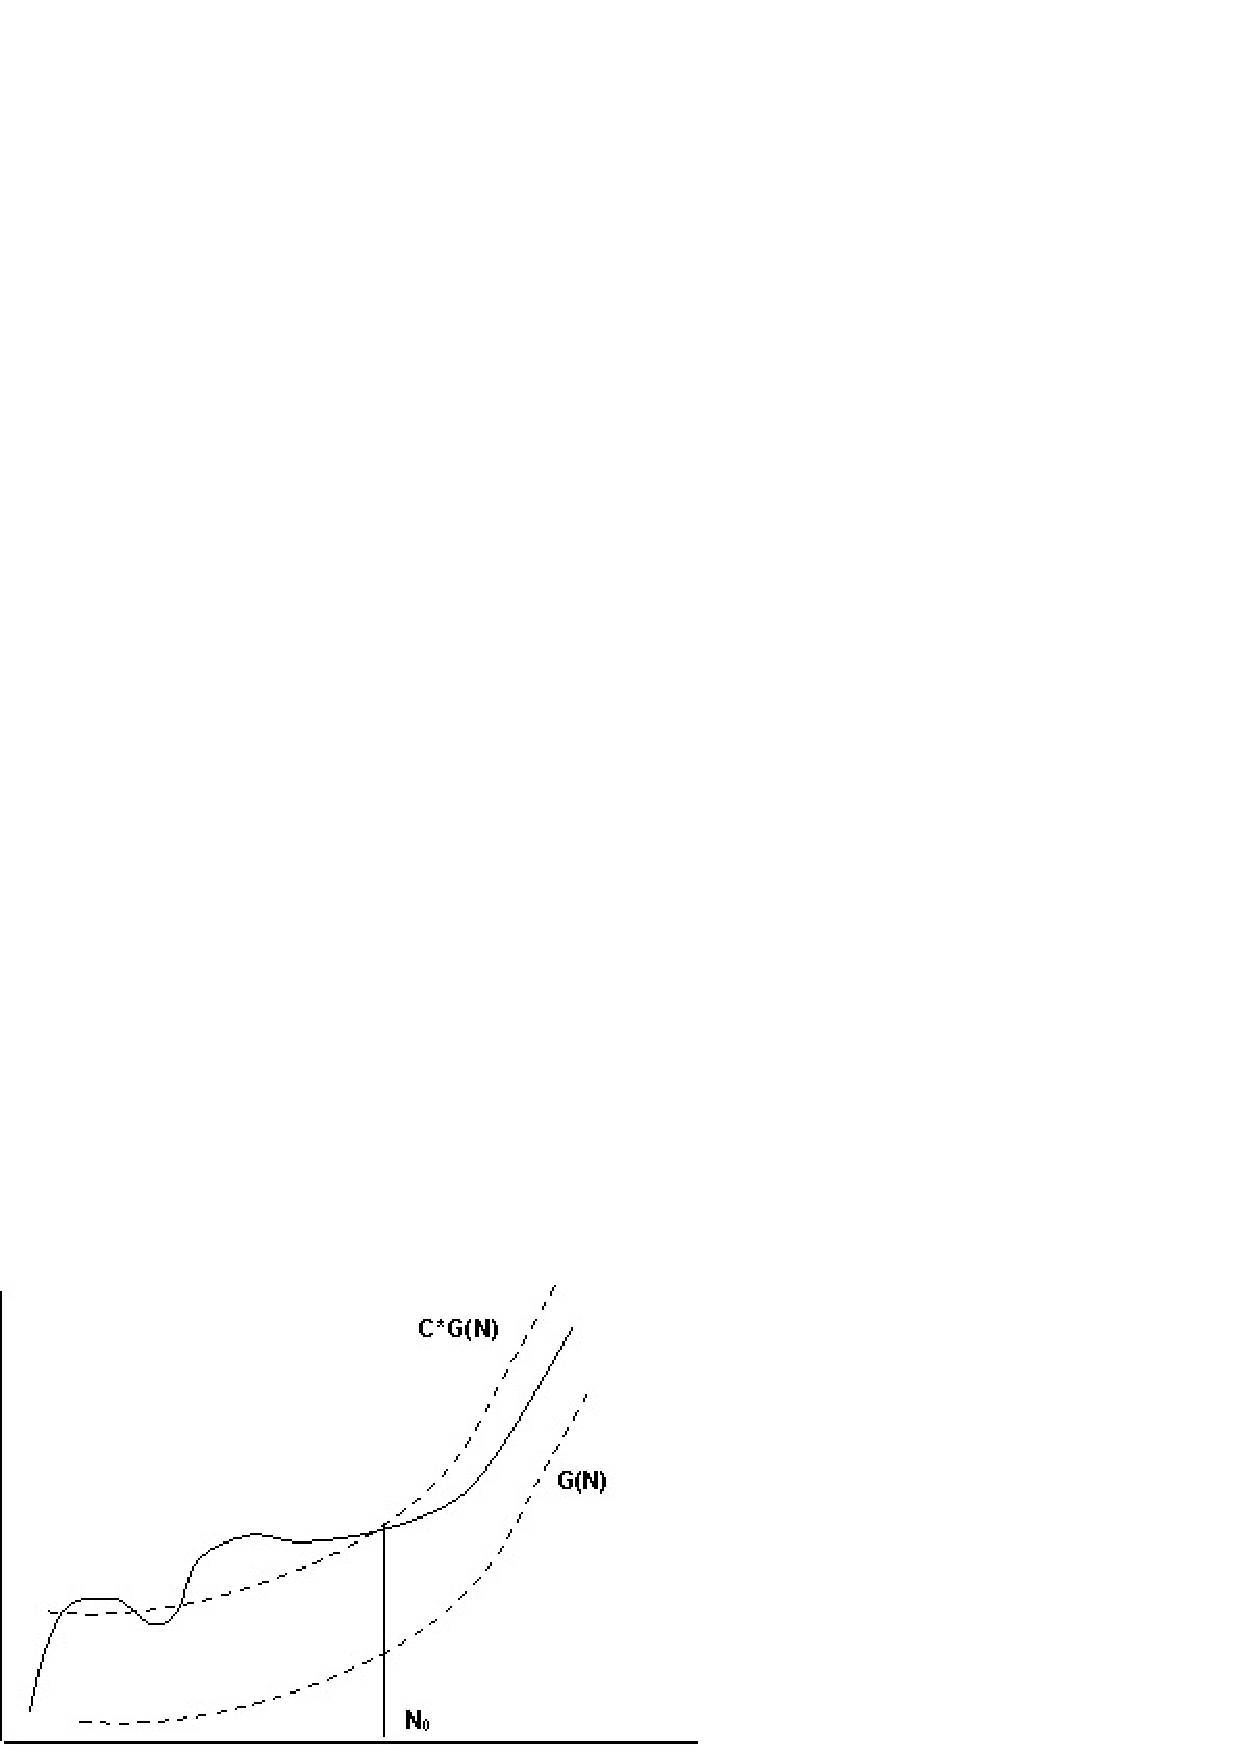
\includegraphics[scale = 0.7]{img/1.png}}
%	\caption{
%		Пример корректной работы}
%	\label{fig:t1}
%\end{figure}

\subsection{Постановка эксперимента}

\begin{enumerate}
	\item Сравнить время работы полного перебора
	и муравьиного алгоритма на 5 матрицах размерностью 10,
	для получения более точного результата произвести
	вычисления над каждой матрицей 10 раз.
	Параметры: $\alpha = 0.5, \rho = 0.5, tmax = 300$.
	\item Выяснить при каких параметрах $\alpha \in [0; 1]$, $\rho \in (0; 1]$, 
	$tmax \in [10; 200]$, где $\alpha, \rho \in \mathbb{R}$, $t \in \mathbb{N}$
	муравьиный алгоритм будет работать лучше. При этом
	значения $\alpha$ и $\rho$ меняются с шагом 0.1, \textit{t\_max} --- с шагом 10.
\end{enumerate}

\subsection{Сравнительный анализ на основе эксперимента}

\subsubsection{Сравнение времени работы}

Замеры произведены на 4-ядерном процессоре \textit{Intel Core i7}
с тактовой частотой 2,4 ГГц, оперативная память --- 8 ГБ.

Экспериментально получена таблица сравнения времени 
(табл. \ref{time1}, время в секундах (с)):

\begin{table} [h!]
	\begin{center}
		\caption{Сравнение времени выполнения алгоритмов решения
			задачи коммивояжера}
		\begin{tabular}{|r|r|r|}
			\hline
			Матрица & Перебор, с & Муравьи, с \\
			\hline
			1 &    24.16445 &   1.737721 \\
			\hline
			2 &    23,37577 &   1,538537 \\
			\hline
			3 &    22,36178 &   1,673532 \\
			\hline
			4 &    25,36118 &   1,80861 \\
			\hline
			5 &    24,35346 &   1,742806 \\
			\hline
		\end{tabular} 
		\label{time1}
	\end{center}
\end{table} 

Видно, что как и ожидалось, муравьиный алгоритм быстрее
решает поставленную задачу --- на экспериментальных
данных в среднем затрачено в 18 раз
меньше времени, чем при полном переборе.

\subsubsection{Параметризация в муравьином алгоритме}

Для проведения параметризации в процессе случайной
генерации получены 5 матриц
размерностью 10, элементы матрицы находятся
в диапазоне от 0 до 100 и кратны 10.

\begin{enumerate}
	\item
	Путь: $( 1 \rightarrow 8 \rightarrow 3 \rightarrow 10 \rightarrow 2 \rightarrow 5 \rightarrow 6 \rightarrow 4 \rightarrow 7 \rightarrow 9 )$
	
	Минимальная длина: 130
	
	\[
	\begin{bmatrix}
	0& 50& 70& 90& 10& 30& 70& 10& 60& 90\\
	50& 0& 60& 60& 10& 80& 40& 10& 80& 80\\
	50& 80& 0& 10& 70& 70& 50& 10& 70& 10\\
	10& 80& 70& 0& 30& 30& 40& 80& 40& 40\\
	40& 20& 50& 20& 0& 10& 10& 70& 20& 20\\
	10& 60& 70& 10& 60& 0& 40& 70& 20& 50\\
	80& 80& 60& 90& 20& 70& 0& 40& 10& 60\\
	50& 30& 10& 60& 50& 10& 50& 0& 10& 90\\
	10& 70& 90& 30& 10& 50& 40& 10& 0& 40\\
	90& 10& 50& 10& 10& 20& 80& 90& 20& 0
	\end{bmatrix}
	\]
	
	\item
	Путь: $( 1 \rightarrow 7 \rightarrow 3 \rightarrow 5 \rightarrow 9 \rightarrow 10 \rightarrow 8 \rightarrow 4 \rightarrow 6 \rightarrow 2 )$
	
	Минимальная длина: 170
	
	\[
	\begin{bmatrix}
	0& 60& 30& 90& 90& 70& 30& 80& 20& 40\\
	10& 0& 10& 50& 70& 70& 20& 20& 60& 40\\
	80& 20& 0& 60& 10& 40& 60& 80& 20& 80\\
	70& 80& 50& 0& 40& 20& 50& 30& 30& 90\\
	90& 20& 10& 80& 0& 50& 80& 70& 20& 30\\
	30& 30& 70& 70& 70& 0& 90& 10& 90& 80\\
	30& 30& 10& 60& 30& 50& 0& 30& 70& 10\\
	70& 60& 30& 10& 10& 50& 50& 0& 90& 80\\
	60& 50& 30& 60& 60& 60& 60& 20& 0& 10\\
	50& 70& 80& 40& 60& 70& 70& 20& 30& 0
	\end{bmatrix}
	\]
	
	\item
	Путь: $( 1 \rightarrow 7 \rightarrow 3 \rightarrow 4 \rightarrow 6 \rightarrow 5 \rightarrow 9 \rightarrow 2 \rightarrow 8 \rightarrow 10 )$
	
	Минимальная длина: 180
	
	\[
	\begin{bmatrix}
	0& 70& 30& 20& 90& 40& 10& 40& 10& 70\\
	70& 0& 30& 10& 80& 80& 20& 20& 40& 30\\
	50& 70& 0& 10& 10& 90& 10& 70& 10& 40\\
	50& 70& 60& 0& 10& 20& 70& 50& 60& 20\\
	30& 80& 10& 90& 0& 10& 10& 20& 10& 30\\
	50& 80& 30& 70& 10& 0& 50& 90& 50& 30\\
	10& 50& 10& 30& 10& 20& 0& 70& 80& 30\\
	20& 70& 10& 30& 30& 30& 90& 0& 10& 20\\
	80& 50& 60& 80& 90& 60& 70& 70& 0& 80\\
	20& 90& 20& 20& 20& 90& 50& 80& 90& 0
	\end{bmatrix}
	\]
	
	\item
	Путь: $( 1 \rightarrow 3 \rightarrow 2 \rightarrow 8 \rightarrow 5 \rightarrow 6 \rightarrow 10 \rightarrow 4 \rightarrow 9 \rightarrow 7 )$
	
	Минимальная длина: 110
	
	\[
	\begin{bmatrix}
	0& 10& 10& 10& 80& 70& 40& 20& 10& 10\\
	20& 0& 60& 70& 70& 80& 40& 10& 90& 10\\
	10& 10& 0& 50& 70& 90& 50& 40& 20& 40\\
	60& 10& 10& 0& 60& 90& 50& 60& 10& 20\\
	60& 60& 60& 20& 0& 10& 10& 10& 30& 70\\
	60& 60& 80& 10& 90& 0& 70& 80& 90& 10\\
	10& 70& 30& 60& 30& 20& 0& 50& 10& 30\\
	40& 10& 80& 80& 10& 50& 60& 0& 70& 30\\
	60& 20& 70& 30& 20& 80& 20& 60& 0& 20\\
	20& 20& 90& 10& 10& 50& 20& 50& 70& 0
	\end{bmatrix}
	\]
	
	\item
	Путь: $( 1 \rightarrow 3 \rightarrow 4 \rightarrow 10 \rightarrow 7 \rightarrow 8 \rightarrow 2 \rightarrow 6 \rightarrow 9 \rightarrow 5 )$
	
	Минимальная длина: 160
	
	\[
	\begin{bmatrix}
	0& 90& 10& 40& 10& 90& 90& 70& 60& 60\\
	70& 0& 90& 50& 40& 10& 40& 90& 50& 50\\
	10& 30& 0& 50& 20& 10& 90& 60& 50& 20\\
	70& 60& 90& 0& 60& 30& 60& 10& 20& 20\\
	10& 10& 90& 60& 0& 30& 70& 40& 60& 50\\
	20& 40& 80& 60& 60& 0& 30& 80& 10& 70\\
	50& 40& 10& 50& 40& 60& 0& 10& 40& 30\\
	60& 20& 50& 80& 70& 70& 50& 0& 10& 40\\
	30& 60& 30& 80& 10& 10& 40& 30& 0& 80\\
	60& 30& 10& 90& 20& 30& 10& 20& 10& 0
	\end{bmatrix}
	\]
	
\end{enumerate}

В таблице \ref{param1} приведен пример соответствия параметров
с полученными результатами для матрицы 1.

\begin{table} [h!]
	\begin{center}
		\caption{Параметризация на матрице 1}
		\begin{tabular}{|r|r|r|r|r|r|}
			\hline
			{\bf №} & {\bf $\alpha$} &  {\bf $\rho$} &    {\bf t} & {\bf Ответ} & {\bf Муравьи} \\
			\hline
			{\bf 0} &        0.0 &        0.1 &       10 &        130 &        190 \\
			\hline
			{\bf 1} &        0.0 &        0.1 &       20 &        130 &        190 \\
			\hline
			{\bf 2} &        0.0 &        0.1 &       30 &        130 &        190 \\
			\hline
			{\bf 3} &        0.0 &        0.1 &       40 &        130 &        190 \\
			\hline
			{\bf 4} &        0.0 &        0.1 &       50 &        130 &        190 \\
			\hline
			{\bf 5} &        0.0 &        0.1 &       60 &        130 &        190 \\
			\hline
			\ldots & \ldots & \ldots & \ldots & \ldots & \ldots\\
			\hline
			{\bf 360} &        0.1 &        0.9 &       10 &        130 &        170 \\
			\hline
			{\bf 361} &        0.1 &        0.9 &       20 &        130 &        170 \\
			\hline
			{\bf 362} &        0.1 &        0.9 &       30 &        130 &        160 \\
			\hline
			{\bf 363} &        0.1 &        0.9 &       40 &        130 &        160 \\
			\hline
			{\bf 364} &        0.1 &        0.9 &       50 &        130 &        160 \\
			\hline
			{\bf 365} &        0.1 &        0.9 &       60 &        130 &        170 \\
			\hline
			\ldots & \ldots & \ldots & \ldots & \ldots & \ldots\\
			\hline
			{\bf 806} &        0.4 &        0.1 &       70 &        130 &        160 \\
			\hline
			{\bf 807} &        0.4 &        0.1 &       80 &        130 &        150 \\
			\hline
			{\bf 808} &        0.4 &        0.1 &       90 &        130 &        150 \\
			\hline
			{\bf 809} &        0.4 &        0.1 &      100 &        130 &        170 \\
			\hline
			{\bf 810} &        0.4 &        0.1 &      110 &        130 &        150 \\
			\hline
			\ldots & \ldots & \ldots & \ldots & \ldots & \ldots\\
			\hline
			{\bf 1517} &        0.7 &        0.6 &        180 &        130 &        190 \\
			\hline
			{\bf 1518} &        0.7 &        0.6 &        190 &        130 &        190 \\
			\hline
			{\bf 1519} &        0.7 &        0.6 &        200 &        130 &        190 \\
			\hline
			{\bf 1520} &        0.7 &        0.7 &         10 &        130 &        190 \\
			\hline
			{\bf 1521} &        0.7 &        0.7 &         20 &        130 &        190 \\
			\hline
			{\bf 1522} &        0.7 &        0.7 &         30 &        130 &        190 \\
			\hline
			\ldots & \ldots & \ldots & \ldots & \ldots & \ldots\\
			\hline
			{\bf 2195} &        1.0 &        1.0 &      160 &        130 &        270 \\
			\hline
			{\bf 2196} &        1.0 &        1.0 &      170 &        130 &        300 \\
			\hline
			{\bf 2197} &        1.0 &        1.0 &      180 &        130 &        270 \\
			\hline
			{\bf 2198} &        1.0 &        1.0 &      190 &        130 &        280 \\
			\hline
			{\bf 2199} &        1.0 &        1.0 &      200 &        130 &        280 \\
			\hline
		\end{tabular}  
		\label{param1}
	\end{center}
\end{table} 

Для остальных матриц получены соответствующие таблицы. Тем
не менее, гораздо удобнее
анализировать результаты в графическом виде.
%На рис. \ref{fig:chart1}-\ref{fig:chart5} приводятся графики
%соответствия ответов при различных параметрах $\alpha$, $\rho$, \textit{t}.

\pagebreak

%\begin{figure}[h!]
%	\center{
%		\includegraphics[width = \textwidth]{chart/chart1.pdf}}
%	\caption{Параметризация на матрице 1}
%	\label{fig:chart1}
%\end{figure}

%\begin{figure}[h!]
%	\center{
%		\includegraphics[width = \textwidth]{chart/chart2.pdf}}
%	\caption{Параметризация на матрице 2}
%	\label{fig:chart2}
%\end{figure}

\pagebreak

%\begin{figure}[h!]
%	\center{
%		\includegraphics[width = \textwidth]{chart/chart3.pdf}}
%	\caption{Параметризация на матрице 3}
%	\label{fig:chart3}
%\end{figure}

%\begin{figure}[h!]
%	\center{
%		\includegraphics[width = \textwidth]{chart/chart4.pdf}}
%	\caption{Параметризация на матрице 4}
%	\label{fig:chart4}
%\end{figure}

\pagebreak

%\begin{figure}[h!]
%	\center{
%		\includegraphics[width = \textwidth]{chart/chart5.pdf}}
%	\caption{Параметризация на матрице 5}
%	\label{fig:chart5}
%\end{figure}

\pagebreak

Значения $\alpha$, $\rho$, \textit{t}, на которых муравьиный
алгоритм показал приемлемый результат для всех 5 выбранных матриц,
представлены в таблице \ref{param2}.

\pagebreak

\begin{table} [h!]
	\begin{center}
		\caption{Результаты параметризации}
		\begin{tabular}{|r|r|r|}
			\hline
			$\alpha$ &       $\rho$ & \textit{t} \\
			\hline
			0.1 &        0.1 &         60 \\
			\hline
			0.1 &        0.2 &         50 \\
			\hline
			0.1 &        0.2 &        180 \\
			\hline
			0.1 &        0.3 &        170 \\
			\hline
			0.1 &        0.9 &         50 \\
			\hline
			0.1 &        0.9 &        150 \\
			\hline
			0.1 &        0.9 &        190 \\
			\hline
			0.2 &        0.2 &         80 \\
			\hline
			0.2 &        0.2 &        200 \\
			\hline
			0.2 &        0.3 &         60 \\
			\hline
			0.2 &        0.3 &        140 \\
			\hline
			0.2 &        0.4 &        190 \\
			\hline
			0.2 &        0.5 &         90 \\
			\hline
			0.2 &        0.5 &        100 \\
			\hline
			0.2 &        0.6 &         90 \\
			\hline
			0.2 &        0.6 &        140 \\
			\hline
			0.2 &        0.6 &        200 \\
			\hline
			0.2 &        0.7 &         10 \\
			\hline
			0.2 &        0.7 &        190 \\
			\hline
			0.2 &        0.8 &         60 \\
			\hline
			0.2 &        0.8 &        180 \\
			\hline
			0.2 &        0.9 &        190 \\
			\hline
			0.2 &        0.9 &        200 \\
			\hline
			0.3 &        0.1 &        140 \\
			\hline
			0.3 &        0.3 &         10 \\
			\hline
			0.3 &        0.9 &        160 \\
			\hline
			0.3 &        1.0 &        110 \\
			\hline
			0.4 &        0.1 &         60 \\
			\hline
			0.4 &        0.1 &        160 \\
			\hline
			0.4 &        0.3 &        110 \\
			\hline
			0.4 &        0.5 &         40 \\
			\hline
			0.4 &        0.6 &        160 \\
			\hline
			0.4 &        0.8 &         60 \\
			\hline
			0.4 &        1.0 &         70 \\
			\hline
		\end{tabular}    
		\label{param2}
	\end{center}
\end{table} 

\pagebreak

\subsection*{Выводы}
\addcontentsline{toc}{subsection}{Выводы}

Можно заметить, что хорошие результаты получены
при $\alpha \in [0,1; 0,4]$ в сочетании с $\rho \in (0; 1]$ и 
$t \in \{50; 150; 200\}$. Однако,
стоит учесть, что для других классов задач
параметры могут иметь совсем не такие значения. Для
каждого отдельного случая необходимо проводить
параметризацию.

\section*{Заключение}
\addcontentsline{toc}{section}{Заключение}

В работе экспериментально подтверждена эффективность
муравьиного алгоритма в сравнении с точным перебором
всех маршрутов (на матрицах размерностью 10 быстрее в 2 раза). Также проведена параметризация вероятностного
алгоритма муравья. Результаты свидетельствуют, что
при $\alpha \in [0,1; 0,4]$ в сочетании с $\rho \in (0; 1]$ и 
$t \in \{50; 150; 200\}$ получаются
приемлемые результаты на случайных матрицах размерностью 10.
Тем не менее,
стоит учесть, что для других классов задач
параметры могут иметь совсем не такие значения. Для
каждого отдельного случая необходимо проводить
новую параметризацию.

\addcontentsline{toc}{section}{Список литературы}
\begin{thebibliography}{7}
	
	\bibitem{stovba}
	Штовба С.Д. Муравьиные алгоритмы // Exponenta Pro. Математика в приложениях, 2003, №4, с.70-75
	
	\bibitem{mcconell}
	Дж. Макконнелл. Анализ алгоритмов. Активный 
	обучающий 
	подход.-М.:Техносфера, 2009.
	
	\bibitem{knuth}
	Д. Кнут. Искусство программирования, М., Мир, 1978
	
	\bibitem{kom}
	Задача коммивояжера  [Электронный ресурс]. – Режим доступа: http://www.math.nsc.ru/LBRT/k5/OR-MMF/TSPr.pdf, свободный – (02.12.2019)
	
	\bibitem{pract}
	Практическое применение алгоритма решения задачи коммивояжера [Электронный ресурс]. – Режим доступа: https://cyberleninka.ru/article/n/prakticheskoe-primenenie-algoritma-resheniya-zadachi-kommivoyazhera/, свободный – (01.12.2019)
	
	\bibitem{ant}
	Алгоритмы муравья [Электронный ресурс]. – Режим доступа: http://www.berkut.mk.ua/download/pdfsmyk/algorMurav.pdf, свободный – (24.11.2019)
	
	\bibitem{opt}
	Оптимизация методом колонии муравьев [Электронный ресурс]. – Режим доступа: https://habr.com/ru/post/163887/, свободный – (28.11.2019)
	
	\bibitem{python}
	Python 3.8.2rc1 documentation [Электронный ресурс]. - Режим доступа: https://docs.python.org/3/, свободный - (28.11.2019)
	
	\bibitem{pycharm}
	PyCharm documentation [Электронный ресурс]. - Режим доступа: https://www.jetbrains.com/pycharm/documentation/ - (28.11.2019)
	
\end{thebibliography}

\end{document}